%\documentclass[letterpaper]{IEEEtran}
\documentclass[letterpaper, conference]{IEEEtran}      % Use this line for a4 paper
%\IEEEoverridecommandlockouts                              %

%\usepackage{mathcomSTEP}

%\overrideIEEEmargins 
%\IEEEoverridecommandlockouts                              % This command is only needed if 
% you want to use the \thanks command

%\overrideIEEEmargins                                      % Needed to meet printer requirements.

% See the \addtolength command later in the file to balance the column lengths
% on the last page of the document

\usepackage{mathptmx} 
\usepackage{times} 
\usepackage{amsmath} 
\usepackage{amsbsy} 
\usepackage{amssymb}
%\usepackage{newtxtext, newtxmath}
\usepackage{mathrsfs}
\usepackage{comment}
\usepackage[export]{adjustbox}
\usepackage{tikz}
\usetikzlibrary{external,positioning,decorations.pathreplacing,shapes,arrows,patterns}

%\tikzexternalize[mode=list and make]
\usepackage{algorithmicx}
\usepackage{pgfplots}
\usepackage{graphicx}
\usepackage{pstool}
\usepackage[latin1]{inputenc}
\usetikzlibrary{arrows,shapes}
\usepackage{xifthen}
\usepackage{epic}
\usepackage{caption}
\usepackage{epstopdf}

\newtheorem{thm}{\bf{Theorem}}
\newtheorem{cor}[thm]{\bf {Corollary}}
\newtheorem{lem}[thm]{\bf {Lemma}}
\newtheorem{prop}[thm]{\bf {Proposition}}
\newtheorem{example}{\bf {Example}}
\newtheorem{definition}{\bf {Definition}}
\newtheorem{rem}{\bf {Remark}}

\newcommand{\mmse}{\mathsf{mmse}}
\newcommand{\supp}{\mathrm{supp} }
\renewcommand\vec[1]{\ensuremath\boldsymbol{#1}}
\newenvironment{proof}{\paragraph*{Proof}}{\hfill$\square$ \newline}
\newcommand{\sgn}{\mathrm{sgn} }
\newcommand{\argmax}{\mathrm{argmax}}
\newcommand*{\QEDA}{\hfill\ensuremath{\square}}


\tikzstyle{int}=[draw, fill=blue!10, minimum height = 1cm, minimum width=1.5cm,thick ]
\tikzstyle{sint}=[draw, fill=blue!10, minimum height = 0.5cm, minimum width=0.8cm,thick ]
\tikzstyle{sum}=[circle, fill=blue!10, draw=black,line width=1pt,minimum size = 0.5cm, thick ]
\tikzstyle{ssum}=[circle, fill=blue!10,draw=black,line width=1pt,minimum size = 0.1cm]
\tikzstyle{int1}=[draw, fill=blue!10, minimum height = 0.5cm, minimum width=1cm,thick ]
\tikzstyle{enc}=[draw, fill=blue!10, minimum height = 2.7cm, minimum width=1cm,thick ]
\tikzstyle{int}=[draw, fill=blue!10, minimum height = 1cm, minimum width=1.5cm,thick ]


\title{\LARGE \bf Mean Estimation from Adaptive Single-bit Measurements}
%
\author{
\IEEEauthorblockN{Alon Kipnis}
\IEEEauthorblockA{Department of Electrical Engineering \\
Stanford University\\
Stanford, CA\\}
\and
\IEEEauthorblockN{John C. Duchi}
\IEEEauthorblockA{Department of Electrical Engineering \\
and Department of Statistics \\
Stanford University\\
Stanford, CA\\}
}

\begin{document}
\graphicspath{{../Figures/}}
\maketitle
\thispagestyle{empty}
\pagestyle{empty}



%%%%%%%%%%%%%%%%%%%%%%%%%%%%%%%%%%%%%%%%%%%%%%%%%%%%%%%%%%%%%%%%%%%%%%%%%%%%%%%%
\begin{abstract}
We consider the problem of estimating the mean of a normal distribution under the constraint: that the estimator can access only a single bit per sample from this distribution. We study the squared error in this estimation as a function of the number $n$ of samples and single-bit measurements in an adaptive setting. We show that if at each stage $n$, this single bit is a function of both the new sample and the previous $n-1$ acquired bits, then no estimator can attain asymptotic squared error smaller than $\pi/(2n)$ times the variance. Therefore, we conclude that a strict bit limitation increases the number of samples required for a prescribed accuracy by a factor of at least  $\pi/2$ compared to the unrestricted case. In addition, we provide an explicit estimator that attains this asymptotic error, showing that, rather surprisingly, only $\pi/2$ times more samples are required in order to attain performance equivalent to the unrestricted case. 
\end{abstract}

%{\color{red}  The $\mu$-sum problem (Kim-ElGamal Ch. 21) gives a lower bound. Can be reduced to the CEO.}

%{\color{red}  See LASSO results in http://arxiv.org/abs/1506.02181v1}

%%%%%%%%%%%%%%%%%%%%%%%%%%%%%%%%%%%%%%%%%%%%%%%%%%%%%%%%%%%%%%%%%%%%%%%%%%%%%%%%
\section{Introduction}
\label{sec:Intro}

Processing and estimating information from data collected at multiple physical location may be subject to communication constraints. 
%For example, emerging sensor network technologies in medicine and ``smart cities" use many low-cost sensors to collect large amounts of data and transmit it to remote locations. These sensors must operate under severe power restrictions, hence they are limited by their communication bandwidth. 
For example, consider large-scale sensor arrays where information is collected at multiple physical locations and transmitted to a central estimation unit. In this scenario, the ability to estimate a particular parameter from data collected by the sensors is dictated not only by quality of observations and their numbers, but also by the constraint on the communication rates between the sensors. The question that we ask is to what extend a parametric estimation task is affected by such communication constraint, and what are the fundamental performance of estimation subject to these restrictions. \\

In this paper we provide an answer to this question in a particular simple setting: the estimation of the mean $\theta$ of a normal distribution with a known variance $\sigma^2$, under the constraint that given the $n$th sample $X_n$, only a single bit can be communicated to the estimator. 
Specifically, the $n$th encoder observes $X_n$ and the $n-1$ previous single bit messages $M_1,\ldots,M_{n-1}$, and delivers a single bit message $M_n$ to the estimator. The estimator provides an estimate $\widehat{\theta}_n$ based on $M^n = (M_1,\ldots,M_n)$. 




 \item[(iii)] \emph{Distributed} encoding: the output of the $n$th encoder is a single bit that is only a function of $X_n$.
 \end{itemize}
Clearly, as far as information sharing is concerned, settings (iii) is a more restrictive version of (ii) which is more restrictive than (i). We measure the estimation performance by the mean squared error (MSE) risk. Since without bit constraint this risk is known to be $\sigma^2/n$, we are interested in particular in the \emph{asymptotic relative efficiency} (ARE) of estimators in the constrained setting, defined as the ratio between their MSE to $\sigma^2/n$ as $n$ goes to infinity.
%\par
%Maybe explain here why the problem is interesting ? 
%setting (i), setting (ii) + SDM, setting (iii) + CEO.
%The turn to 1) main results and 2) other previous works. 
%
\par
Classical works on statistical estimation under communication constraint in information theory \cite{720540, zhang2013information, zhang1988estimation} implies that the ARE in setting (i) is $1$. Namely, asymptotically, there is no loss in performance in this setting due to the communication constraint. Indeed, under setting (i) the sample mean can be described by an encoder with an exponentially decaying error, leading to MSE of $\sigma^2/n + o(2^{-n})$. In this work we show that a similar result does not hold even in setting (ii): the relative efficiency of any adaptive estimator is at least $\pi/2$. Namely, the single-bit per sample constraint incurs a minimal penalty of at least $\approx 1.57$ compared to an unconstrained estimator or to the optimal estimator in setting (i). In addition to this negative statement, we provide an estimator that almost surely attains this minimal relative efficiency. In other words, we show that the lower bound of $\pi/2$ on the asymptotic relative efficiency is tight, and that it is attained regardless of the particular realization of $\theta$ or the size of the parameter space from which it is taken. Clearly, the minimal penalty on the efficiency of $\pi/2$ also holds under setting (iii), although the question whether such efficiency is achievable (or otherwise, what is the minimal efficiency) remains open. \\


\subsection{Relate Works}
The parametric estimation problem we consider is closely related to many works in statistics and information theory. Statistical inference under multiterminal data compression \cite{han1987hypothesis, zhang1988estimation} includes as a special case the problem of estimating a single vector of parameters from multiple data-rate constrained observations. These inference problems were studied in the asymptotic limit as the number of observations goes to infinity. In this asymptotic setting the unconstrained inference performance is always attained when all samples are taken from the same distribution \cite[Sec. III]{720540}. Indeed, in an i.i.d setting the \emph{type} of the sample is a sufficient statistics for any estimation task, and the latter can be described using a number of codewords polynomial in $n$ regardless of the distribution of the samples. For this reason in \cite{han1987hypothesis} and \cite{zhang1988estimation} attention is given to inference problems involving multiple distributions observed at different locations. Setting (i) above can be seen as a special case of the above works where the communication is limited to a single-bit per terminal. In fact, with a full access to the sample prior to encoding, the problem of encoding and estimating $\theta$ is reduced to the MSE attained by a scalar quantizer adjusted to the sufficient statistics of the sample \cite{gray1998quantization}.
%On the other hand, setting (iii) arises as the number of terminals grow with $n$ and their communication rates are limited to a single bit. 

This last situation is also obtained by the multiterminal source coding setting, a.k.a. the CEO problem \cite{berger1996ceo} can be seen as a generalization of our setting (iii), where multiple draws of $\theta$ and rounds of $n$ bit communication is permitted. In particular, the minimal CEO distortion with $1$ bit per terminal provides a lower bound on the MSE risk.  

In fact, with a full access to the sample as in setting (i), the problem of encoding and estimating $\theta$ is reduced to the MSE attained by a scalar quantizer adjusted to the sufficient statistics of the sample \cite{gray1998quantization}. The sigma-delta modulatior (SDM) \cite{1092194} uses a single bit quantizer with a feedback loop, and therefore falls under setting (ii). The SDM with a constant input $\theta$ corrupted by a Gaussian noise was considered in \cite{53738}, where it was shown that the output of the modulator converges to the true constant input. Therefore, the SDM provides a consistent estimator for setting (ii). The rate of this convergence, however, was not analyzed and cannot be derived directly from the results of \cite{53738}. In fact, the results of this paper implies that the rate of convergence of a SDM to a constant input signal is at most $\sigma^2\pi/2$ over the number of feedback iterations. \par


%
Estimation problem subject to the one-bit quantization constraint were also considered in compressed sensing \cite{boufounos20081,baraniuk2017exponential} and in MIMO detection in wireless communication \cite{singh2009limits}. 


The rest of this paper is organized as follows: the main problem and notation are defined in Section~\ref{sec:problem}. In Section~\ref{sec:sequential} we present a lower bound on estimation from one-bit samples in the adaptive scheme, as well as an achievable scheme that attains this bound. Concluding remarks are given in Section~\ref{sec:conclusions}.



\section{Motivation and Related Works}
Standard considerations implies that the optimal encoding in setting (i) is reduced to an optimal $n$ bits description of the  sample mean. The standard technique to encode an unknown random quantity using $n$ bits is attained by an optimal scalar quantizer. However, the design of this quantizer depends on the distribution of its input \cite{gray1998quantization}, which is the goal of the estimation. Therefore, although the ARE in this setting is shown to be one \cite[Sec. III]{720540}, we see that a non-trivial challenge arise even in this case. 
In setting (ii), the above challenge of optimal quantizer design with imprecise input distribution occurs upon the the arrival of each new sample $X_n$. 

%sigma delta modulator

%implies the existence of a consistent estimator in this case

% our result provides a lower bound for the accuracy of a sigma-delta modulator 



Setting (ii) and (iii) were considered in 
\cite{zhang2013information} under the more general assumption of $m$ machines each has access to $n/m$ independent samples. The main result of \cite{zhang2013information} are lower bounds on the estimation error as a function of the total number of bits $R$ with which each machine can communicate. Our settings corresponds to the case $m=n$ and $R=1$, and our result is a fundamental lower bound and a matching achievable scheme under this simplified setting. 

 We also note that the counterpart of setting (iii) in the case of hypothesis testing was considered in \cite{52470}. 



 The optimal design  requires the distribution of the input, which is the goal of estimation and is known appriori. 

 standard technique to encode an unknown random quantity using $n$ bits is attained by an optimal scalar quantizer,  by designing a scaler quantizer Unlike standard quantization task of encoding an unn

%Note that when multiple realization of $\theta$ are involved, the prior distribution $P_\theta$ plays a significant role in the overall MSE, whereas in our case we expect the final distortion to be independent of the actual prior distribution as in the two schemes in the sequential case. \\




\subsection{Intuition from Remote Multiterminal Source Coding}
A first clue for this rather surprising result can be seen drawing the connection between our parametric estimation problem to the remote multiterminal source coding problem of \cite{berger1996ceo}, also known as the CEO problem. The CEO setting considers $n$ encoders, each has access to a corrupted version of a source signal. The $i$th encoder observes $k$ noisy source symbols and transmit $R_i k$ bits to a central estimator. Therefore, assuming that $\theta$ is drawn randomly from a prior $\pi(\theta)$, the distributed estimation setting (iii) corresponds to the CEO setting with $k=1$, where the $i$th agent observes 
\begin{equation}
\label{eq:Gaussian_channel}
X_i = \theta + Z_i,
\end{equation}
and has $R_i=1$ bits to transmit this observation. As a result, the quadratic distortion in the optimal source coding scheme for the CEO with $n$ terminals at rates $R_1 = \ldots = R_n = 1$ and Gaussian observation noise of variance $\sigma^2$ provides a lower bound on the MSE distortion in estimating $\theta$. In fact, the difference between this lower bound and the actual MSE in our setting indicates the importance of coding over blocks consisting of $k$ independent realizations of $\theta$ versus $k=1$ in our setting. \par
A closed-form expression for CEO under quadratic distortion is known only for the case where the sequence to described by the encoders is sampled from a Gaussian distribution \cite{prabhakaran2004rate}. By using the characterization of the minimal CEO distortion as the number of terminals goes to infinity, we conclude the following:
\begin{prop} \label{prop:ceo_lower_bound}
Assume that $\pi(\theta)$ is the normal distribution. Then any estimator $\widehat{\theta}_n$ of $\theta$ in the distributed setting satisfies
\[
 n\mathbb E \left( \theta - \theta_n \right)^2 \geq \frac{4\sigma^2}{3} + o(1).
\]
\end{prop}

\begin{proof}
We consider the expression \cite[Eq. 10]{chen2004upper} that provides the minimal distortion $D^\star$ in the CEO with $L$ observers and under a total sum-rate $R_\Sigma = R_1 + \ldots R_L$:
\begin{equation} \label{eq:ceo_optimal_sumrate}
R_{\Sigma} = \frac{1}{2} \log^+ \left[ \frac{\sigma_\theta^2}{D^\star} \left( \frac{D^\star L}{ D^\star L - \sigma^2 + D^\star \sigma^2 / \sigma_\theta^2 }\right)^L  \right].
\end{equation}
Assuming $R_\Sigma = n$ and $L=n$ we get
\begin{equation} \label{eq:ceo_optimal_sumrate}
n = \frac{1}{2} \log \left[ \frac{\sigma_\theta^2}{D^\star} \left(\frac{ D^\star n }{D^\star n - \sigma^2 + D^\star \sigma^2/\sigma_\theta^2 }  \right)^n  \right].
\end{equation}
The value of $D^\star$ that satisfies the equation above describes the MSE in the quadratic Gaussian CEO setting under an optimal allocation of the sum-rate $R_\Sigma = n$ among the $n$ encoders. Therefore, $D^\star$ provides a lower bound to the CEO distortion with $R_1=\ldots,R_n = 1$ and hence a lower bound to the minimal MSE in estimating $\theta$ in the distributed setting. By considering $D^\star$ in \eqref{eq:ceo_optimal_sumrate} as $n\rightarrow \infty$ we conclude that 
\[
D^\star = \frac{ \frac{4\sigma^2}{3} }{n + \frac{4 \sigma^2}{3 \sigma_\theta^2} } + O(e^{-n}) =  \frac{4\sigma^2}{3n} + o(n^{-1}). 
\]
\end{proof}
We note that although the CEO lower bound was derived by the MSE attainable assuming optimal allocation a total of $n$ bits among the encoders, the same expression is from the upper bound to the CEO derived in \cite[Prop. 5.2]{KipnisRini2017}, that assumes $R_1=\ldots,R_n = 1$ rather than optimal allocation of $n$ bits among all encoders. %\[
%D_{CEO} / \sigma_\theta^2 \leq \left( 1 + \sum_{i=1}^n \frac{\sigma_\theta^2}{\sigma^2} \frac{1 - 2^{-2R_i}} {1+ \frac{\sigma_\theta^2}{\sigma^2}  2^{-2 R_i}  } \right)^{-1}
%\]
%where $\sigma_\theta^2$ is the variance of the distribution $\pi(\theta)$. Using $R_1=\ldots=R_n=1$ we get
%\[
%D_{CEO} \leq  \left( \frac{1}{\sigma_\theta^2} +  \frac{3n}{4\sigma^2 + \sigma_\theta^2} \right)^{-1}   =
%\frac{4 \sigma^2}{3n} +  \frac{\sigma_\theta^2}{3n} + o(n^{-1}). 
%\]



Statistical inference problems under communication constraints in the nature of our setting were considered in information theory in 
\cite{han1987hypothesis, zhang1988estimation, 720540}. These works consider a multi-terminal source coding setting in which the $i$th terminal observes $n$ samples from the distribution and is allotted $nR_i$ bits to communicate its estimate. The main focus of these works is the difference between inference with communication constraint and the unconstrained vanilla statistical estimation setting, as the number of samples $n$ goes to infinity subject to a total finite rate constraint. Our setting (i) can be seen as a special case of this setting where with a single terminal and $R_1 = 1$.% whereas our case (iii) is obtained from this setting by taking $n=1$, $R_i=1$, and number of terminals grow with $n$. 
However, as explained in \cite[Sec. III]{720540}, a single terminal in this setting always lead to the unconstrained inference performance. Indeed, when all samples are taken from the same distribution, the \emph{type} of the sample \cite{csiszar1998method} is a sufficient statistics for any inference task, and the latter can be described using a number of codewords polynomial in $n$ regardless of the distribution of the samples. For this reason, attention is given in these works to inference problems involving multiple distributions observed at different locations and hence the results there do not apply to our setting. In fact, with a full access to the sample as in setting (i), the problem of encoding and estimating $\theta$ is reduced to the MSE attained by a scalar quantizer adjusted to the sufficient statistics of the sample. Finally, we note that setting (ii) includes as a special case the sigma-delta modulation (SDM) analog-to-digital conversion scheme with a constant input $\theta$ corrupted by Gaussian noise $Z_i$, as was considered in \cite{53738}. While it was shown there that the output of the modulator converges to the true constant input, the rate of this convergence was not analyzed and cannot be derived directly from the results of \cite{53738}. In fact, a corollary from the results in this paper we conclude that the rate of convergence of a SDM to a constant input signal is at most $\sigma^2\pi/2$ over the number of feedback iterations. Finally, the multiterminal source coding setting denoted as the CEO problem \cite{berger1996ceo} can be seen as a generalization of our setting (iii), where multiple draws of $\theta$ and rounds of $n$ bit communication is permitted. In particular, the minimal CEO distortion with $1$ bit per terminal provides a lower bound on the MSE risk.  \par


%Why it is surprising that the estimator is independent of $\theta$, $\Theta$ or $\pi(\theta)$. 


\subsection{Related Works}
\subsubsection*{Statistical inference under communication constraints}
The problem of statistical inference under communication constraint has a long and rich history in statistics and information theory. Statistical inference under multiterminal data compression \cite{han1987hypothesis, zhang1988estimation} includes as a special case the problem of estimating a single vector of parameters from multiple data-rate constrained observations. These inference problems were studied in the asymptotic limit as the number of observations goes to infinity. The main question asked there is the difference between inference with communication constraint and the unconstrained vanilla statistical estimation setting. In this asymptotic setting the unconstrained inference performance is always attained when all samples are taken from the same distribution \cite[Sec. III]{720540}. Indeed, in an i.i.d setting the \emph{type} of the sample is a sufficient statistics for any estimation task, and the latter can be described using a number of codewords polynomial in $n$ regardless of the distribution of the samples. For this reason in \cite{han1987hypothesis} and \cite{zhang1988estimation} attention is given to inference problems involving multiple distributions observed at different locations. Setting (i) above can be seen as a special case of \cite{han1987hypothesis, zhang1988estimation, 720540} where the communication is limited to a single-bit per terminal. 

%\subsubsection{Estimation from 1-bit measurements}
%Single-bit or binary detectors are the basis for digital technology, and works considers the estimation of parameters from the results of such detectors have been around from the early days of digital computing. The burst of works in compressed sensing in the previous decade also gave raise to multiple 1-bit results \cite{rice_university}. Due to the popularization of MIMO technology and the expected break of mm-wave in wireless communication there have been many works 1-bit detection at the A/D in the receiver \cite{2016arXiv160204193Z}. 

\subsubsection*{Relation to channel coding}
The problem we consider is the estimation of the parameter $\theta$ by observing 
\begin{equation}
\label{eq:channel}
X_i = \theta + Z_i, \quad i=1,\ldots,n,
\end{equation}
where the $Z_i$s are independent, centered normal with variance $\sigma^2$. The problem of estimating $\theta$ from the $X_i$s can be seen as the attempt to transmit a real number $\theta$ over an additive white Gaussian noise (AWGN) channel. In particular, setting (ii) can be seen as the feedback version of this transmission, which is closely related to \cite{horstein1963sequential, 1053879}. However, in our setting $\theta$ is either fixed or drawn once from a prior distribution, so the communication in \eqref{eq:channel} is limited to a repetition code. Moreover, in setting (ii) we have the additional constraint that the message is a causal function of the previous messages, where in case (iii) it is completely memoryless. Works in information theory which consider such setting includes AWGN channel with 1-bit ADC at the receiver \cite{DBLP:journals/corr/VarastehSG16}. \par

\subsubsection*{Relation to source coding}
With a full access to the sample as in setting (i), the problem of encoding and estimating $\theta$ is reduced to the MSE attained by a scalar quantizer adjusted to the sufficient statistics of the sample. Setting (ii) includes as a special case the sigma-delta modulation (SDM) analog-to-digital conversion scheme with a constant input $\theta$ corrupted by Gaussian noise $Z_i$, as was considered in \cite{53738}. While it was shown there that the output of the modulator converges to the true constant input, the rate of this convergence was not analyzed and cannot be derived directly from the results of \cite{53738}. As a corollary from the results in this paper we conclude that the rate of convergence of a SDM to a constant input signal is at most $\sigma^2\pi/2$ over the number of feedback iterations. Finally, the remote multiterminal source coding setting of \cite{berger1996ceo} corresponds to the case of $n$ rate-constrained encoders, each observing a noisy version of an information source. The difference between this setting and ours is that in ours the parameter of interest is not an information source. By assuming a prior distribution on this parameter, the CEO provides a lower bound on the estimation error in the fully distributed setting (iii). This lower bound can be attained if we were to consider the average error in multiple independent realizations of our problem rather than a single realization as we do here. \\

%As opposed to the aforementioned line of works, we focus on estimation of samples taken from a single distribution in the finite blocklength performance. We are interested in particular in addition restrictions on the communication and information sharing between the encoders. For example, our main focus is the case where the observer must communicate a single bit upon drawing from the distribution. This is in contrast to the asymptotic setting where the observer can encode the outcome of $n$ draws at once using a single $n$ bit message. Alternately, such setting can be seen as having $n$ different observers, each is capable of observing a single realization and transmit a single bit. 

%{\color{red} The Van Trees inequality was extended to the estimation of multiple parameters in \cite{bobrovsky1987}. It is closely related with the }

\begin{comment}
\subsection{Sigma-Delta Encoding}

and covariance function \cite[Eq. 25]{53738}
\[
R(k) = \mathbb E M_{n+k} M_n = \theta^2 + O \left( \frac{1}{\sigma \sqrt{ k} } \right). 
\]
{\color{red} This is not enough to deduce convergence. Need to go over the paper and check if rate of convergence can be deduced. Also do simulations BEFORE that. \\

What is the error in estimating the mean of stationary ergodic process ? 
}
Since the SDM is a special case of the sequential scheme, we conclude that the MSE of any SDM with a noisy DC signal is bounded from below by $n^{-1} \sigma^2 \pi/2 $.
\end{comment}


The rest of this paper is organized as follows: the main problem and notation are defined in Section~\ref{sec:problem}. Our main results are presented and discussed in Section~\ref{sec:sequential}. Concluding remarks are given in Section~\ref{sec:conclusions}.


%Even with such arguably simple setting, we will see that the performance limit in the estimating task based on single bit observations provides an interesting setting for discussion that bridges classical works in statistics, coding theory, information theory and optimization. 


\section{Problem Formulation \label{sec:problem}}

\begin{figure}
\begin{center}
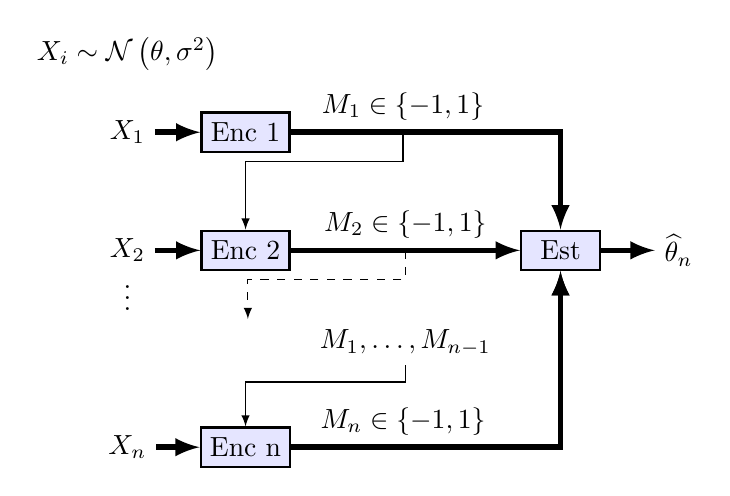
\begin{tikzpicture}[node distance=2cm,auto,>=latex]
  \node at (0,0) (source) {$X_1$} ;
  \node[int1, right of = source, node distance = 1.5cm] (enc1) {Enc 1};  
\draw[->,line width = 2pt] (source) -- (enc1); 

 \node[below of = source, node distance = 1.5cm] (source2) {$X_2$};
\node[int1, right of = source2, node distance = 1.5cm] (enc2) {Enc 2};  
\draw[->,line width = 2pt] (source2) -- (enc2); 

\node[below of = source2, node distance = 2.5cm] (source3) {$X_n$};
\node[int1, right of = source3, node distance = 1.5cm] (enc3) {Enc n};  
\draw[->,line width = 2pt] (source3) -- (enc3); 


\node[above of = source, node distance = 1cm] (dist) {$X_i \sim {\mathcal N} \left(\theta, \sigma^2 \right)$};
\node[below of = source2, node distance = 0.5cm] {$\vdots$};

\node[int1, right of = enc2, node distance = 4cm ] (est) {Est};
\draw[->,line width = 2pt] (enc1) -| node[above, xshift = -2cm] (mes1) {$M_1 \in \left\{-1,1\right\}$} (est);   
\draw[->,line width = 2pt] (enc2) -- node[above, xshift = 0cm] (mes2) {$M_2 \in \left\{-1,1\right\}$} (est);   
\draw[->] (mes1) -- +(0,-0.7) -| (enc2);

\draw[dashed,->] (mes2) -- +(0,-0.7) -| +(-2,-1.2);
\draw[->,line width = 2pt] (enc3) -| (est);   

\node[below of = mes2, node distance = 1.5cm] (mes3) {$M_1,\ldots,M_{n-1} $};

\draw[->,line width = 2pt] (enc3) -| node[above, xshift = -2cm]  {$M_n \in \left\{-1,1\right\}$} (est);   

\draw[->] (mes3) -- +(0,-0.5) -| (enc3);

\node[right of = est, node distance = 1.5cm] (dest) {$\widehat{\theta}_n$};
%         \node [int1] (dec) [right of=dest, node distance = 1.5cm,  align=center] {\small Dec };
%\node [int1] (enc) [right of = dec, node distance = 3cm]{Enc}; 
%\draw[->,line width=2pt] (dec) -- (dest);
\draw[->, line width=2pt] (est) -- (dest);
\end{tikzpicture}
\end{center}
\caption{\label{fig:sequential} Adaptive single-bit encoding: the $i$th encoder delivers a single bit message which is a function of its private sample $X_i$ and the previous messages $M_1,\ldots,M_{i-1}$.}
\end{figure}

Let $X_i$, $i=1,\ldots,n$, be $n$ independent samples from the normal distribution $\mathcal N(\theta,\sigma^2)$ with mean $\theta$ and variance $\sigma^2$. We assume that the mean $\theta$ is drawn once from a prior distribution $\pi(\theta)$ on the parameter space $\Theta$, which is a closed interval of the real line. We moreover assume that $\pi(\theta)$ is absolutely continuous with respect to the Lebesgue measure with density $\pi(d\theta)$. The problem we consider is the estimation of the parameter $\theta$ under the following constraints on the communication between the samples $X_1,\ldots,X_n$ and a centralized estimator: 
\begin{itemize}
\item[(i)] The estimator at time $n$ is only a function of the $n$ messages $M^n = \left(M_1,\ldots,M_n \right)$.
\item[(ii)] For each $i=1,\ldots,n$, the $i$th message $M_i$ is a function of the sample $X_i$ and the $i-1$ previous messages $M^{i-1}$.
\item[(iii)] The $i$th message $M_i$ takes only two possible values, say $1$ and $-1$. 
\end{itemize}
In other words,  the $n$ messages $M^n$ are the only information on the sample $X^n = \left(X_1,\ldots,X_n\right)$ available to the estimator. The $i$th message is defined by a function from the real line to $\{-1,1\}$, measurable with respect to the sigma algebra generated by $M^{i-1}$ and $X_i$.  The estimator, upon observing $M^n$, produces an estimate $\widehat{\theta}_n(M^n)$ of $\theta$. A system describing the above scheme is illustrated in Fig.~\ref{fig:sequential}. \\

In this work we are concerned with the mean squared error (MSE) risk:
\begin{equation}
\label{eq:error_def}
\epsilon_n \triangleq \mathbb E\left(\widehat{\theta}_n - \theta \right)^2,
\end{equation}
where the expectation is taken with respect to the distribution of $X^n$ and the prior distribution $\pi(\theta)$. \\
%It is well known that minmax estimation error 
%\begin{equation}
%E_n = \min \sup_{\theta \in \Theta}  \mathbb E\left[ \left(\widehat{\theta}_n - \theta \right)^2 | \theta \right],
%\end{equation}
%can be obtained from $\epsilon_n$ by assuming a particular least favorable prior distribution on the parameter space $\Theta$ \cite{casella1981}. 

The main problem we consider is the minimal value that can be attain in \eqref{eq:error_def} as a function of $n$. Note that this minimization is the combination of the following two procedures: (1) selecting the $i$th message $M_i$ based on past messages and current observation $X_i$, and (2) estimating $\theta$ given messages $M^n$. We are interested in particular in the asymptotic relative efficiency of estimators $\widehat{\theta}_n$ for $\theta$ compared to the sample mean $\bar{X}_n = \frac{1}{n} \sum_{i=1}^n X_i$. Since the MSE attained by the latter is $\sigma^2/n$, this relative efficiency is defined as
\begin{equation}
\rho \triangleq \lim_{n \rightarrow \infty} \frac{n}{\sigma^2}  \epsilon_n. 
\label{eq:relative_efficiency}
\end{equation}
{\color{red}
Since the conditional expectation of $\theta$ with respect to $\bar{X}_n$ (and not $\bar{X}_n$) minimizes \eqref{eq:error_def}, we need to justify the fact that we use the sample mean as the reference estimator.
}

In addition to the notations defined above, we denote by $\phi(x)$ the standard normal density and by $\Phi(x)$ the standard normal cumulative distribution function. Prime denote derivative with respect to $\theta$.

% Lower Bound on the assymptotic minimal effeciency.
% Scheme that attains the assymptotic minimal effeciency. 
% Bayesian scheme that is one step optimal. We leave open the question whether this scheme attains the asymptotic minimal effeciency 

\section{Results \label{sec:sequential}}
The first main results of this paper, as described in Theorem~\ref{thm:adpative_lower_bound} below, states that the asymptotic relative efficiency of and adaptive estimator cannot get below $\pi/2$. Next, we provide a particular adaptive estimation scheme and show in Theorem~\ref{thm:sgd} that its efficiency is $\pi/2$. Finally, in Theorem~\ref{thm:opt_one_step} we provide an adaptive estimation scheme that is optimal in the sense that at each step $i$, the message $M_i$ that minimizes the MSE given $X_i$ and the previous $M^{i-1}$ messages is chosen. While it is not clear whether the efficiency of this last scheme is $\pi/2$, numerical simulations suggests that the MSE of this scheme time s $n$ converges as well to $\pi/2$, but in a faster rate than the first scheme. 

%While we provide expressions for the optimal message, evaluating the asymptotic efficiency of this estimation scheme turns out to be a challenging task. We therefore leave open the question whether this scheme attains the lower bound with equality, and only provide numerical result that support this conjecture.  \\

%\begin{figure}
%\begin{center}
%\begin{tikzpicture}[node distance=2cm,auto,>=latex]
%  \node at (0,0) (theta) {$\theta$} ;
%  \node at (2,0) (x1) {$X_1$};
%  \node[below of = x1, node distance = 1cm] (x2) {$X_2$};
%    \node[below of = x2, node distance = 1cm] (dots) {$\vdots$};
%  \node[below of = dots, node distance = 1cm] (xn) {$X_n$};
%  
%   \node[right of = x1, node distance = 2cm] (m1) {$M_1$};
%  \node[right of = x2, node distance = 2cm] (m2) {$M_2$};
%    \node[right of = xn, node distance = 2cm] (mn) {$M_n$};
%
%\draw[->] (theta) -- (x1);
%\draw[->] (theta) -- (x2);
%\draw[->] (theta) -- (xn);
%
%\draw[->] (x1)--(m1);
%\draw[->] (x2)--(m2);
%\draw[->] (xn)--(mn);
%
%\draw[->] (m1)--(m2);
%\draw[->, dashed] (m2)--(mn); 
%  
%\end{tikzpicture}
%\end{center}
%\caption{\label{fig:sequencial_graphical} Graphical model notation of the sequential setting.}
%\end{figure}

%\subsection{Properties of an Optimal Scheme}
%The sequential nature of the encoding and the estimation is best explain by the notions of actions and rewards taken from dynamic programming. The \emph{action} taken by the $i$th encoder is the design of a detection region $M_i^{-1}(1)$ that would lead to $M_i = 1$ assuming when $X_i \in M_i^{-1}(1)$ or $M_i=-1$ otherwise. The \emph{reward} (or penalty) is only evaluated at the end of the time horizon $n$.
%% Dynamic program. State = $M^n$. 
%% Reward is collected at the end
%% 

\subsection{A Lower Bound on Adaptive Single-Bit Schemes}
Our first results asserts that the relative efficiency \eqref{eq:relative_efficiency} of any adaptive estimation scheme is bounded from below by $\pi/2$, as follows from the following theorem:
\begin{thm}[minimal relative effeciency] \label{thm:adpative_lower_bound}
Let $\widehat{\theta}_n$ be any estimator of $\theta$ in the adaptive setting of Fig.~\ref{fig:sequential}.
% Let $\pi(\theta)$ be an absolutely continuous prior distribution on $\Theta$ with density function converges to zero at the endpoints of the interval $\Theta$. 
Assumes that $P(d\theta)$ converges to zero at the endpoints of the interval $\Theta$. Then
\[
\mathbb E (\theta-\theta_n)^2 \geq  \frac{\pi \sigma^2 }{2n +\pi \sigma^2  I_0}  =  \frac{\pi}{2n}\sigma^2+o(n^{-1}),
\]
where 
\[
I_0 = \mathbb E \left( \frac{d}{d\theta} \log P_\theta(\theta) \right)^2
\]
is the Fisher information with respect to a location model in $\theta$. 
\end{thm}

\subsubsection*{Sketch of Proof}
The main idea in the proof is to bound from above the Fisher information of any set of $n$ single-bit messages with respect to $\theta$. Once this bound is achieved, the result follows by using the Van-Trees inequality \cite{gill1995applications} which bounds from below the MSE of any estimator of $\theta$ by the inverse of the expected value of the aforementioned Fisher information plus $I_0$. The details are given in the Appendix.\\

Next, we present an adaptive estimation scheme which attains the minimal asymptotic efficiency $\pi/2$. 
%Theorem~\ref{thm:adpative_lower_bound}. This estimation scheme can be seen as a gradient descent 

\subsection{Asymptotically Optimal Estimator}
Consider the following estimator $\widehat{\theta}_n$ for $\theta$:  set 
\begin{equation}
\label{eq:sgd_alg}
\theta_n = \theta_{n-1} +  \gamma_n \sgn (X_n - \theta_n), \quad n = 1,2,\ldots,
\end{equation}
where $\left\{\gamma_n \right\}_{n=1}^\infty$ is any strictly positive sequence satisfying 
\begin{enumerate}
\item[(i)] $\frac{\gamma_n - \gamma_{n+1}}{\gamma_n} = o(\gamma_n)$ \\
\item[(ii)] $\sum_{n=1}^\infty \frac{\gamma_n^{(1+\lambda)/2}} {\sqrt{n}} < \infty$ 
for some $0< \lambda \leq 1$.
\end{enumerate}
(e.g. $\gamma_n = n^{-\beta}$ for $\beta \in (0,1)$). The $n$th step estimation is defined by 
\begin{equation} \label{eq:sgd_est}
\widehat{\theta}_n =  \frac{1}{n} \sum_{i=1}^n  \theta_i. 
\end{equation}

As the following theorem shows, the estimator $\widehat{\theta}_n$ defined by \eqref{eq:sgd_est} and \eqref{eq:sgd_alg} attains the minimal asymptotic efficiency as established by Theorem~\ref{thm:adpative_lower_bound}.
\begin{thm} \label{thm:sgd}
The sequence $\widehat{\theta}_n$ of \eqref{eq:sgd_alg} satisfies
\[
\sqrt{n} \left( \widehat{\theta}_n - \theta \right) \overset{d}{\rightarrow} \mathcal N \left(0,  \pi \sigma^2 /2 \right).
\]
\end{thm}

\subsubsection*{Proof}
The asymptotic behavior of \eqref{eq:sgd_est} is a special case of  \cite[Thm. 4]{polyak1992acceleration}. The details are provided in the Appendix.\\


Note that $\theta_0$ is not explicitly defined in 
in equation \eqref{eq:sgd_est}. Arguably, a reasonable initialization is $\theta_0 = \mathbb E [\theta]$. However, Theorem~\ref{thm:sgd} implies that the asymptotic behavior of the estimator, is indifferent to this initialization. Thus, the optimal efficiency is attained without using the prior distribution on $\theta$. Nevertheless, the bound in Theorem~\ref{thm:adpative_lower_bound} suggests that the estimation error can be greatly reduced whenever the prior of $\theta$ provides a lot of information $I_0$ on its location. In order to incorporate this information in a more meaningful way, we present a Bayesian estimation scheme that is conjectured to attain the optimal asymptotic efficiency. 

\subsection{One-step Optimal Estimation}
In this subsection we present an estimation scheme that posses the property of \emph{one-step optimality}. That is, at each step $i$, the $i$th encoder designs the detection region $M_i^{-1}(1)$ such that the MSE given $M^i$ is minimal. In other word, this scheme designs the messages in a greedy manner, such that the MSE at step $i$ is minimal given the current state of the estimation described by $M^{i-1}$. \\

The structure of the message that minimizes the next step MSE is given by the following theorem:
\begin{thm}[optimal one-step estimation] \label{thm:opt_one_step}
Let $\pi(\theta)$ be an absolutely continuous log-concave probability distribution. Given a sample $X$ from the distribution $\mathcal N(\theta, \sigma^2)$, define 
\begin{equation}
\label{eq:adaptive_main_message}
M = \sgn(X - \tau),
\end{equation}
where $\tau$ satisfies the equation
\begin{equation}
 \label{eq:fixed_point}
 \tau = \frac{m^-(\tau) + m^+(\tau)}{2},
\end{equation}
with
\begin{align*}
m^-(\tau)  & = \frac{\int_{-\infty}^{\tau} \theta P(d\theta) }{\int_{-\infty}^{\tau} P(d\theta)} ,\\
m^+(\tau) & = \frac{\int_{\tau}^\infty \theta P(d\theta) }{\int_{\tau}^\infty P(d\theta)} .
\end{align*}
Then for any estimator $\widehat{\theta}$ which is a function of $M'(X) \in \{-1,1\}$, we have
\begin{equation}
\label{eq:opt_cond}
\mathbb E \left(\theta-\widehat{\theta}(M')\right)^2 \geq  \mathbb E \left(\theta- \mathbb E[\theta|M]\right)^2,
\end{equation}
\end{thm}

\begin{proof}
The proof is completed by the following two lemmas, proofs of which can be found in the Appendix:
\begin{lem} \label{lem:unique}
Let $f(x)$ be a log-concave probability density function. Then the equation 
\begin{equation}
\label{eq:lem_fixed_point}
2x = \frac{\int_x^\infty uf(u)du}{\int_x^\infty f(u)du} + \frac{\int_{-\infty}^x uf(u)du}{\int_{-\infty}^x f(u)du} 
\end{equation}
has a unique solution.
\end{lem}
\end{proof}

\begin{lem} \label{lem:adaptive}
Let $U$ be an absolutely continuous random variable with
pdf $P(du)$. Then the one-bit message $M^\star$ that minimizes
\[
\int \left( u - \mathbb E[U|M(u)]  \right)^2 P(du)
\]
is given by
\[
M^\star  =  \sgn(U - \tau),
\]
where $\tau$ is the unique solution to the equation
 \[
2 \tau = \frac{\int_{\tau}^\infty u P(du)} {\int_{\tau}^\infty P(du)} + \frac{\int_{-\infty}^{\tau} u P(du)}{\int_{-\infty}^{\tau} P(du)}.
\]
\end{lem}

Theorem~\ref{thm:opt_one_step} suggests the following Bayesian estimation scheme: set $P_0(t) = \pi(\theta)$, and for $n\geq 1$ update the prior as
\begin{align}
P_n(t) = & P(\theta=t |M^n) = \frac{ P\left( \theta=t | M^{n-1} \right) P(M_n | \theta = t , M^{n-1})  } { P(M_n | M^{n-1} )} \nonumber \\ 
& = \alpha_n  P_{n-1}(t) \Phi\left(M_n \frac{ t - \tau_{n-1} }{\sigma} \right), \label{eq:density_update}
\end{align}
where $\alpha_n$ is a normalization coefficient that equals to
\[
\alpha_n = \left(\int_{\mathbb R} P_{n-1}(t) \Phi\left(M_n \frac{t- \tau_{n-1} }{\sigma} \right)  dt \right)^{-1}. 
\]
The $n$th estimate for $\theta$ is the conditional expectation of $\theta$ given $M^n$, namely
\begin{equation}
\theta_n = \mathbb E \left[ \theta| M^n\right] = \int_{-\infty}^\infty t P_n(t) dt. \label{eq:estimator_update}
\end{equation}
Next, solve equation \eqref{eq:fixed_point} with the updated prior $P_n(t)$ instead of $P(\theta)$. Note that since the standard normal cdf $\Phi(x)$ is log-concave, the updated prior $P_n(t)$ remains log-concave and thus a unique solution to \eqref{eq:fixed_point} is guaranteed by Lemma~\ref{lem:unique}. Finally, update the $n+1$th message as
\begin{equation}\label{eq:message_update}
M_{n+1} = \sgn(X_{n+1}-\tau_n).
\end{equation}

Since the equation \eqref{eq:fixed_point} has no analytic solution in general, it is hard to derive the asymptotic behavior of the Bayes estimator defined by \eqref{eq:estimator_update} and \eqref{eq:message_update}. We conjecture, however, that it attains the asymptotic relative efficiency of $\sigma^2\pi/2$, as can be observed from the numerical simulation illustrated in Fig.~\ref{fig:adaptive_error}. Also shown in Fig.~\ref{fig:adaptive_error} are the normalized MSE of the estimator defined by \eqref{eq:sgd_alg} and \eqref{eq:sgd_est}, as well as the MSE achieved by the sample mean for the same sample realization. 

 % In fact, the numerical simulation in Fig.~\ref{fig:simulation} shows that this scheme outperform the estimator of \eqref{eq:sgd_est} even when the prior on $\Theta$ is least favorable for Bayes estimation \cite{Bickel1981}. 


\begin{figure}
\begin{center}
\begin{tikzpicture}
\node at (0,0) {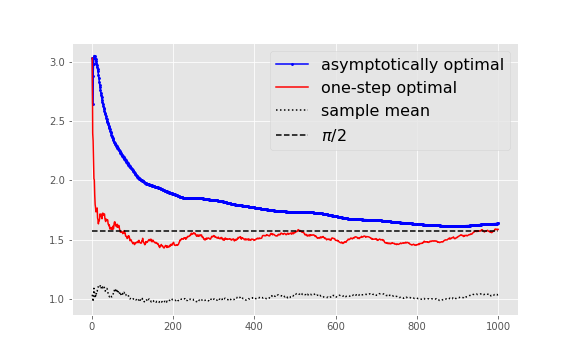
\includegraphics[scale=0.4]{error}};
\end{tikzpicture}
\caption{Normalized empirical risk $n\left(\widehat{\theta}_n-\theta\right)^2$ versus number of samples $n$ for $100$ Monte Carlo trials. In each trial, $\theta$ is chosen uniformly in the interval $(-5,5)$. \label{fig:adaptive_error}  }
\end{center}
\end{figure}


\begin{comment}
\subsection{Relation to Sigma-Delta Modulation \label{subsec:sdm}}
The SDM is a device that converts continuous-time analog signals to a discrete-time sequence of binary digits. The basic operation of a SDM can be described as follows: the modulator takes as input a sequence of continuous amplitude samples $X_n$, which are typically represents samples of a continuous-time signal taken uniformly at sampling rate $f_s$ much higher than the Nyquist rate of the signal \cite{1095151}. The output of the modulator is a sequence $M_n$ of binary values, obtained according to the following rule: 
\begin{align}
\begin{cases} V_{n+1} & =  V_n - \alpha q(V_n) + X_n, \\
M_n & = \sgn(V_n)  \end{cases}, \quad n=1,2,\ldots, \label{eq:sdm}
\end{align}
where $\alpha > 0$ is a parameter of the modulator that is determined by the maximal value of the input sequence $X^n$. The SDM of the form \eqref{eq:sdm} was studied in \cite{53738} under the assumption that the input process $X_n$ is an i.i.d Gaussian process. The main results from \cite{53738} shows that regardless of the initial state $V_0$, the process $M_n$ is a stationary ergodic process with mean $\theta$. It follows that a consistent estimation of $\theta$ is obtained by taking the mean of the sequence $\{M_n\}$. However, the results from \cite{53738} does not provide a closed form for the second order statistics of $\{M_n\}$, so that convergence rate cannot be derived from \cite{53738}.  
\end{comment}


\section{Conclusions \label{sec:conclusions}}
We considered the relative efficiency in estimating the mean of a normal distribution from single-bit measurements in an adaptive setting. We have shown that this minimal relative efficiency is $\pi/2$, namely there is a penalty factor of at least $\pi/2$ on the asymptotic MSE in estimating the mean compared to an estimator that has full access to the sample. We also showed that this lower bound is tight by presenting an estimation procedure that attains it.
%but ignores the prior distribution on the parameter space.
In addition, we characterized the single-bit message that minimizes the next step MSE, and described an estimation procedure that is based on a sequence of one-step optimal messages. We leave open the questions whether this estimator attains the minimal efficiency and whether it leads to an estimation scheme which is globally optimal. \\

%Something about how to interpret the results

% Sigma-Delta
% Relation to CEO
% Open questions
% Extenstion to fully distributed setting

\section*{ACKNOWLEDGMENT}
This research is supported in parts by...
%Tsachy Weissman, Stefano Rini, Robert Gray.

\onecolumn

\appendix

\section{Proofs}
In this appendix we provide detailed proofs of our main results as described in Section~\ref{sec:sequential}.

\subsection*{Proof of Theorem~\ref{thm:adpative_lower_bound}}

We first prove the following two lemmas:
\begin{lem} \label{lem:bound_intervals}
For any $x_1 \geq \ldots \geq x_n \in \mathbb R$, we have 
\begin{equation}
\frac{ \left(  \sum_{k=1}^n (-1)^{k+1}\phi(x_k) \right)^2} 
{\left( \sum_{k=1}^n (-1)^{k+1} \Phi(x_k) \right)\left(1- \sum_{k=1}^n (-1)^{k+1} \Phi(x_k) \right)  } \leq \frac{2} {\pi}. \label{eq:bound_intervals}
\end{equation}
\end{lem}
\begin{lem} \label{lem:fisher_bound}
Let $X\sim \mathcal N(\theta,\sigma^2)$ and assume that 
\[
M(X) = \begin{cases} 1,& X \in A, \\
-1, & X \notin A.
\end{cases}
\]
Then the Fisher information of $M$ with respect to $\theta$ is bounded from above by $2/(\pi \sigma^2)$.
\end{lem}

\subsubsection*{Proof of Lemma~\ref{lem:bound_intervals}}
We use induction on $n \in \mathbb N$. For the base case $n=1$ we have 
\begin{equation} \label{eq:induction_base}
\frac{  \phi^2(x)} 
{\Phi(x) \left(1 - \Phi(x) \right) } 
\end{equation}. 
Taking the logarithm of \eqref{eq:induction_base} and differentiating, we conclude that any point $x$ that maximizes \eqref{eq:induction_base} satisfies
\[
x = \phi(x) \left( \Phi(x) -\frac{1}{2} \right).
\]
However, since $x > \phi(x) \left( \Phi(x) -\frac{1}{2} \right)$ for all $x > 0$, the only point that satisfies the last condition is $x=0$. At this point \eqref{eq:induction_base} equals $2/\pi$. \par
Assume now that \eqref{eq:bound_intervals} holds for all integers up to some $n = N-1$ and consider the case $n = N$. The maximal value of \eqref{eq:bound_intervals} is attained for the same $(x_1,\ldots,x_N) \in \mathbb R^N$ that attains the maximal value of 
\begin{align*}
& g(x_1,\ldots, x_N) \triangleq 2 \log \left(  \sum_{k=1}^{N} (-1)^{k+1} \phi(x_k) \right) - \log
\left( \sum_{k=1}^N (-1)^{k+1} \Phi(x_k) \right)
-\log \left(1 -  \sum_{k=1}^N (-1)^{k+1} \Phi(x_k) \right) \\
& = 2 \log \delta_N - \log \Delta_N - \log \left(1 - \Delta_N  \right),
\end{align*}
where we denoted $\delta_N \triangleq \sum_{k=1}^{N} (-1)^{k+1} \phi(x_k)$ and $\Delta_N =  \sum_{k=1}^N (-1)^{k+1} \Phi(x_k)$. The derivative of $g(x_1,\ldots,x_N)$ with respect to $x_k$ is given by
\[
\frac{\partial  g}{\partial x_k} = \frac{2 (-1)^{k+1} \phi'(x_k)}{\delta_N} -\frac{(-1)^{k+1} \phi(x_k)}{\Delta_N } + \frac{(-1)^{k+1} \phi(x_k)}{1-\Delta_N }.
\]
Using the fact that $\phi'(x) = -x \phi(x)$, we conclude that the gradient of $g$ vanishes only if
\[
x_k = \frac{\delta_N}{2} \left( \frac{1}{\Delta_N} - \frac{1}{1-\Delta_N} \right),\quad k=1,\ldots,N.
\]
In particular, the condition above implies $x_1 = \ldots = x_N$. If $N$ is odd then for $x_1=\ldots =x_N$ we have that \eqref{eq:bound_intervals} equals
\[
\frac{\phi(x_1)^2}{ \Phi(x_1) (1 - \Phi(x_1))},
\]
which was shown to be smaller than $\pi/2$. If $N$ is even, then for any constant $c$ the limit of \eqref{eq:bound_intervals} exits as $(x_1,\ldots,x_N)\rightarrow (c,\ldots,c)$ and equals zero. Therefore, the maximum of \eqref{eq:bound_intervals} is not attained at this line. We now consider the possibility that \eqref{eq:bound_intervals} is maximized at the borders, as one or more of the coordinates of $(x_1,\ldots,x_N)$ approaches plus or minus infinity. For simplicity we only consider the cases where $x_N$ goes to minus infinity or $x_1$ goes to plus infinity (the general case where the first $m$ coordinates goes to infinity or the last $m$ to minus infinity is obtained using similar arguments). Assume first $x_N \rightarrow -\infty$. Then  \eqref{eq:bound_intervals} equals
\begin{align*}
\frac{ \left(  \sum_{k=1}^{N-1} (-1)^{k+1}\phi(x_k) \right)^2} 
{\left( \sum_{k=1}^{N-1} (-1)^{k+1} \Phi(x_k) \right)\left(1- \sum_{k=1}^{N-1} (-1)^{k+1} \Phi(x_k)  \right) } ,
\end{align*}
which is smaller than $2/\pi$ by the induction hypothesis. Assume now that $x_1 \rightarrow \infty$. Then 
\eqref{eq:bound_intervals} equals
\begin{align*}
& \frac{ \left(  \sum_{k=2}^{N} (-1)^{k+1}\phi(x_k) \right)^2} 
{\left( 1 + \sum_{k=2}^{N} (-1)^{k+1} \Phi(x_k) \right)\left(1- 1 - \sum_{k=2}^{N} (-1)^{k+1} \Phi(x_k)  \right) }  \\
& = \frac{ \left(  -\sum_{m=1}^{N} (-1)^{m+1}\phi(x'_m) \right)^2} 
{\left( 1 - \sum_{m=1}^{N-1} (-1)^{m+1} \Phi(x'_{m}) \right)\left( \sum_{m=1}^{N-1} (-1)^{m+1} \Phi(x'_{m})  \right) },
\end{align*}
where $x'_{m} = x_{m+1}$. The last expression is also smaller than $2/\pi$ by the induction hypothesis. This proves Lemma~\ref{lem:bound_intervals}. \\

\subsubsection*{Proof of Lemma~\ref{lem:fisher_bound}}
The Fisher information of $M$ with respect to $\theta$ is given by
\begin{align}
I_\theta & =  \mathbb E \left[ \left( \frac{d}{d\theta} \log P\left( M | \theta \right) \right)^2 |\theta \right] \nonumber \\
& = \frac{ \left(\frac{d}{d\theta} P(M=1|\theta) \right)^2}{P(M=1| \theta)} + \frac{ \left(\frac{d}{d\theta} P(M=-1|\theta) \right)^2} {P(M=-1| \theta)} \nonumber \\
& \overset{(a)}{=} \frac{ \left( - \int_A \phi' \left( \frac{x-\theta}{\sigma} \right)dx \right)^2} {\sigma^2 P(M=1| \theta) } + \frac{ \left( \int_A \phi' \left( \frac{x-\theta}{\sigma} \right)dx \right)^2} { \sigma^2P(M=-1| \theta) } \nonumber \\ 
& = \frac{\left( \int_A \phi'\left( \frac{x-\theta}{\sigma} \right) dx \right)^2 }{  \sigma^2 P(M=1 | \theta) \left(1-P(M=1|\theta) \right)  }, \nonumber \\
& = \frac{\left( \int_A \phi'\left( \frac{x-\theta}{\sigma} \right) dx \right) \left( \int_A \phi'\left( \frac{x-\theta}{\sigma} \right) dx \right)}{  \sigma^2 \left( \int_A \phi \left( \frac{x-\theta}{\sigma} \right) dx \right)  \left(1- \int_A \phi \left( \frac{x-\theta}{\sigma} \right) dx \right) }, \label{eq:lem_fisher_bound_proof1}
\end{align}
where differentiation under the integral sign in $(a)$ is possible since $\phi(x)$ is differentiable with absolutely integrable derivative $\phi'(x) = -x\phi(x)$. Regularity of the Lebesgue measure implies that for any $\epsilon>0$, there exists a finite number $k$ of disjoint open intervals $I_1,\ldots I_k$ such that 
\[
\int_{A\setminus \cup_{j=1}^k I_j }  dx < \epsilon \sigma^2,
\]
which implies that for any $\epsilon' > 0$, the set $A$ in \eqref{eq:lem_fisher_bound_proof1} can be replaced by a finite union of disjoint intervals without increasing $I_\theta$ by more than $\epsilon'$. It is therefore enough to proceed in the proof assuming that $A$ is of the form
\[
A = \cup_{j=1}^k (a_j,b_j),
\]
with $\infty \leq a_1 \leq \ldots a_k$, $b_1 \leq b_k \leq \infty$ and $a_j \leq b_j$ for $j=1,\ldots,k$. Under this assumption we have
\begin{align*}
\mathbb P(M_n=1) & = \sum_{j=1}^k \mathbb P\left(X_n \in (a_j,b_j) \right)  \\
& = \sum_{j=1}^k \left( \Phi \left(\frac{b_j-\theta}{\sigma} \right) -  \Phi \left(\frac{a_j-\theta}{\sigma} \right)  \right),
\end{align*}
so \eqref{eq:lem_fisher_bound_proof1} can be rewritten as
\begin{align}
& =   \frac { \left( \sum_{j=1}^{k} \phi \left(\frac{a_j-\theta}{\sigma} \right) - \phi \left( \frac{b_j-\theta} {\sigma} \right)  \right)^2 } 
{\sigma^2 \left( \sum_{j=1}^k \Phi \left( \frac{b_j-\theta }{\sigma}\right) - \Phi \left( \frac{a_j-\theta }{\sigma}\right)  \right) }  \nonumber \\
& \times \frac {1} 
{1- \left( \sum_{j=1}^k \Phi \left( \frac{b_j-\theta }{\sigma}\right) - \Phi \left( \frac{a_j-\theta }{\sigma}\right)  \right) } 
\label{eq:lemma_J}
\end{align}
The proof of Lemma~\ref{lem:fisher_bound} is completed since it follows from~\ref{lem:bound_intervals} that for any $\theta \in \mathbb R$ and any choice of the intervals endpoints, \eqref{eq:lemma_J} is smaller than $2/(\sigma^2 \pi)$. \\


We now consider the proof of Thm.~\ref{thm:adpative_lower_bound}. In order to bound from above the Fisher information of any set of $n$ single-bit messages with respect to $\theta$, we first note that without loss of generality, each message $M_i$ can be written in the form
\begin{equation}
\label{eq:general_messages}
M_i = \begin{cases}
X_i \in A_i & 1, \\
X_i \notin A_i & -1,
\end{cases} 
\end{equation}
where $A_i \subset \mathbb R$ is a Lebesgue measurable set. Indeed, any measurable function $M(X_i) \in \{-1,1\}$ can be written in the form \eqref{eq:general_messages} with $A_i = M^{-1}(1)$. Consider the conditional distribution $P({M^n|\theta})$ of $M^n$ given $\theta$. We have 
\begin{align}
P\left( M^n | \theta \right) & =  \prod_{i=1}^n P\left(M_i | \theta, M^{i-1} \right), \label{eq:adpt_lower_bound_proof:1}
\end{align}
where $P\left(M_i =1 | \theta, M^{i-1}  \right) = \mathbb P\left( X_i \in A_i\right)$. We now prove the following Lemma:



Going back to \eqref{eq:adpt_lower_bound_proof:1}, it follows that the Fisher information of $M^n$ with respect to $\theta$ is given by 
\begin{align}
I_\theta(M^n) = \sum_{i=1}^n I_\theta (M_i|M^{i-1}),
\label{eq:fisher_information}
\end{align}
where $I_\theta (M_i|M^{i-1})$ is the Fisher information of the distribution of $M_i$ given $M^{i-1}$. From Lemma~\ref{lem:fisher_bound} it follows that $I_\theta (M_i|M^{i-1}) \leq 2/(\pi \sigma^2)$. The Van Trees inequality \cite{van2004detection, gill1995applications} now implies 
\begin{align*}
\mathbb E \left( \theta_n - \theta \right)^2 &  \geq \frac{1}{ \mathbb E I_\theta(M^n) + I_0} \\
& = \frac{1}{ \sum_{i=1}^n I_\theta (M_i | M^{i-1} ) + I_0} \\
& \geq \frac{1}{ 2n/(\pi \sigma^2) + I_0}.
\end{align*}

\QEDA

\subsection*{Proof of Theorem~\ref{thm:sgd}}
The algorithm given in \eqref{eq:sgd_alg} and \eqref{eq:sgd_est} is a special case of a more general class of estimation procedures given in \cite{polyak1992acceleration}. In particular, Theorem~\ref{thm:sgd} is follows directly from the following simplified version of \cite[Thm. 4]{polyak1992acceleration}:
\begin{thm}{\cite[Thm. 4]{polyak1992acceleration}} \label{thm:polyak_juditsky}
Let 
\[
X_i = \theta + Z_i,\quad i=1,\ldots,n.
\]
Define 
\begin{align*}
\theta_i & = \theta_{i-1} + \gamma_i \varphi(X_i - \theta_{i-1}), \\
\widehat{\theta}_n & = \frac{1}{n} \sum_{i=0}^{n-1} \theta_i,
\end{align*}
where the $Z_i$s are $\mathcal N(0,\sigma^2)$ and independent of each other, the sequence $\left\{ \gamma_i \right\}_{i=1}^\infty$ satisfies conditions (i) and (ii) in Theorem~\ref{thm:sgd}, and $\left| \varphi(x) \right| \leq K_1(1+x)$ for some $K_1$. Define $\psi(x) = \mathbb E \varphi(x+Z_1)$, $\chi(x) = \mathbb E \varphi^2(x+Z_1)$ and assume that $\psi(0)=0$, $x\psi(x) >0$ for all $x\neq 0$, $\chi(x)$ is continuous at zero, and that $\psi(x)$ is differentiable at zero with $\psi'(0)>0$. Moreover, assume that there exists $K_2$ and $0<\lambda \leq 1$ such that
\[
\left| \psi(x) - \psi'(0)x \right|\leq K_2 |x|^{1+\gamma}.
\]
Then $\widehat{\theta}_n \rightarrow \theta$ almost surely and $ \sqrt{n}(\widehat{\theta}_n - \theta)$ converges in distribution to $\mathcal N(0,V)$, where
\[
V = \frac{ \chi(0)} {\psi'^2(0)}. 
\]
\end{thm}


Using the notation in Theorem~\ref{thm:polyak_juditsky}, we set $\varphi(x) = \sgn(x)$ and $Z_i = X_i - \theta$. We have: 
\[
\chi(x) = \mathbb E \varphi^2(x+Z_1),
\]
so $\chi(0) = 1$. In addition,
\begin{align*}
\psi(x) & = \mathbb E \sgn(x+ Z_1) = \int_{-\infty}^\infty \sgn(x+z) \frac{1}{\sqrt{2\pi}\sigma} e^{-\frac{z^2}{\sigma^2}} dz \\
& = \int_{-x}^\infty \frac{1}{\sqrt{2\pi}\sigma} e^{-\frac{z^2}{\sigma^2}} dz -\int_{-\infty}^{-x} \frac{1}{\sqrt{2\pi}\sigma} e^{-\frac{z^2}{\sigma^2}} dz.
\end{align*}
This leads to 
\begin{align*}
\psi'(x) & = \frac{1}{\sqrt{2\pi}\sigma} e^{-\frac{x^2}{\sigma^2}} dz +\frac{1}{\sqrt{2\pi}\sigma} e^{-\frac{z^2}{\sigma^2}} dz,
\end{align*}
so $\psi'(0) = \frac{2}{\sqrt{2\pi}\sigma}$. It is now easy to verify that the rest of the conditions in Theorem~\ref{thm:polyak_juditsky} are fulfilled for any $\lambda > 0$. Since 
\[
\frac{\chi(0)}{\psi'^2(0)} = \frac{\pi \sigma^2}{2},
\]
Theorem~\ref{thm:sgd} follows from Theorem~\ref{thm:polyak_juditsky}. \QEDA


\subsection*{Proof of Theorem~\ref{thm:opt_one_step}}
In this subsection we prove lemmas \ref{lem:adaptive} and \ref{lem:unique} which lead to Theorem~\ref{thm:opt_one_step}. 

\subsubsection*{Proof of Lemma \ref{lem:adaptive}}
Since any single-bit message $M(u) \in \{0,1\}$ is characterized by two decision region $A_1 = M^{-1}(1)$ and $A_{-1} = M^{-1}(-1)$, it follows that $\mathbb E \left[ U | M(U) \right]$ assumes only two values: $\mu_1 = \mathbb E \left[ U | M(U) = 1 \right]$ and $\mu_{-1} = \mathbb E \left[ U | M(U) = -1 \right]$. We claim that a necessary condition for $M(u)$ to be optimal is that the sets $A_1$ and $A_{-1}$ are, modulo a set of measure $P(du)$ zero, the Voronoi sets on $\mathbb R$ corresponding to the points $\mu_1$ and $\mu_{-1}$, respectively. Indeed, assume by contradiction that for such an optimal partition there exists a set $B \subset A_{1}$ with $\mathbb P (U \in B) >0$ such that $\left( b-\mu_{1} \right)^2 > \left( b- \mu_{-1} \right)^2$. The expected square error in this partition satisfies:
\begin{align*}
& \int_{\mathbb R} \left( u - \mathbb E[U|M(u)]  \right)^2 P(du) = \int_{A_1} (u- \mu_1)^2 P(du) + \int_{A_{-1}} (u- \mu_{-1})^2 P(du) \\
& = \int_{A_1\setminus B} (u- \mu_1)^2 P(du) +  \int_{B} (u- \mu_1)^2 P(du) + \int_{A_{-1}} (u- \mu_{-1})^2 P(du) \\
& > \int_{A_1\setminus B} (u- \mu_1)^2 P(du) +  \int_{B} (u- \mu_2)^2 P(du) + \int_{A_{-1}} (u- \mu_{-1})^2 P(du),
\end{align*}
so clearly, the partition $A_1' = A_1 \setminus B$, $A_{-1}' = A_{-1} \cup B$ attains lower error variance which contradicts the optimality assumption and proves our claim. It is evident that Voronoi partition of the real line corresponding to $\mu_1$ and $\mu_{-1}$ is of the form $A_{-1} = (-\infty,\tau)$, $A_{1} = (\tau, \infty)$ where the point $\tau$ is of equal distance from $\mu_1$ and $\mu_{-1}$, namely $\tau = \frac{\mu_1 + \mu_{-1}}{2}$. From these two conditions (which are a special case of the conditions derived in \cite{1056489} for two quantization regions) we conclude that $\tau$ must satisfy the equation
\[
2 \tau = \frac{\int_{\tau}^\infty u P(du)}{\int_{\tau}^\infty P(du)} + \frac{\int_{-\infty}^{\tau} u P(du)}{\int_{-\infty}^{\tau} P(du)}.
\] 
\QEDA

\subsubsection*{Proof of Lemma \ref{lem:unique}} 
Any solution to \eqref{eq:lem_fixed_point} is a solution to $h^+(x) = h^-(x)$ where
\[
h^+(x) = \frac{\int_x^\infty uf(u)du}{\int_x^\infty f(u)du} - x 
\]
and
\[
h^-(x) = x - \frac{\int_{-\infty}^x uf(u)du}{\int_{-\infty}^x f(u)du}.
\]
We now prove that $h^+(x)$ is monotonically decreasing while $h^-(x)$ is increasing, so they meet at most at one point. The derivative of $h^-(x)$ is given by
\begin{equation} 
\label{eq:one_step_proof_derivative}
1 - \frac{ f(\tau) \int_{-\infty}^\tau f(x) (\tau-x)dx } {\left( \int_{-\infty}^\tau f(x) dx \right)^2}.
\end{equation}
Denote $F(x) = \int_{-\infty}^x f(u)du$. Using integration by parts in the numerator and from the fact that $\lim_{\tau \rightarrow -\infty}  \tau \int_{-\infty}^\tau f(x) dx = 0$, the last expression can be written as
\[
1- \frac{ f(\tau) \int_{-\infty}^\tau F(x) dx}
 {\left( F(\tau) \right)^2}.
\]
Log-concavity of $f(x)$ implies log-concavity of $F(x)$, so that we can write $F(x) = e^{g(x)}$ for some concave and differentiable function $g(x)$. Moreover, we have $f(x) = g'(x)e^{g(x)}$ where, by concavity of $g(x)$, the derivative $g'(x)$ of $g(x)$ is non-increasing. With these notation we have
\begin{align*}
\frac{ f(\tau) \int_{-\infty}^\tau F(x) dx}
 {\left( F(\tau) \right)^2} & = \frac{g'(\tau)e^{g(\tau)} \int_{-\infty}^\tau e^{g(x)}dx }{ e^{2g(\tau)} } \\
 & = e^{-g(\tau)} \int_{-\infty}^\tau g'(\tau) e^{g(x)} dx  \\
 & \leq e^{-g(\tau)} \int_{-\infty}^\tau g'(x) e^{g(x)} dx \\
 & = e^{-g(\tau)} F(\tau) = 1.
\end{align*}
(where the second from the last step follows since $g'(x) \leq g'(\tau)$ for any $x\leq \tau$). If follows that \eqref{eq:one_step_proof_derivative} is non-negative and thus $h^-(x)$ is monotonically increasing. Since
\[
h^+(-x) = x - \frac{ \int_{-\infty}^{x} uf(-u)du}{ \int_{-\infty}^x f(-u) du }, 
\]
the fact that $h^+(x)$ is monotonically decreasing follows from similar arguments. Moreover, since the derivatives of $h^+(x)$ and $h^-(x)$ never vanish at the same time over any open interval, their difference cannot be constant over any interval. Finally, since 
\begin{align*}
 \lim_{x\rightarrow -\infty} h^+(x) =  \lim_{x\rightarrow \infty} h^-(x)
\end{align*}
and since non of these functions are constant, monotonicity of $h^+(x)$ and $h^-(x)$ implies that they must meet at some $x\in \mathbb R$. \QEDA



%%%%%%%%%%%%%%%%%%%%%%%%%%%%%%%%%%%%%%%%%%%%%%%%%%%%%%%%%%%%%%%%%%%%%%%%%%%%%%%%
\bibliographystyle{IEEEtran}
\bibliography{IEEEabrv,/Users/Alon1/LaTex/bibtex/sampling}


\end{document}
